% Wireframe - Comandos de Voz da Integração Alexa
\begin{figura}{Wireframes - Comandos de voz da integração Alexa}{O Autor}
\centering
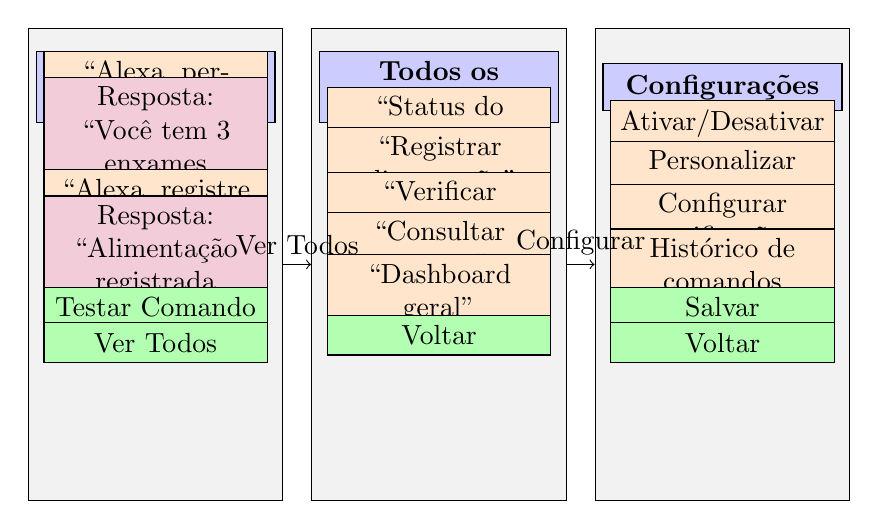
\begin{tikzpicture}[scale=0.9]
% Definição de estilos
\tikzset{
  phone/.style={rectangle, draw, fill=gray!10, text width=3cm, text centered, minimum height=6cm},
  header/.style={rectangle, draw, fill=blue!20, text width=2.8cm, text centered, minimum height=0.6cm},
  button/.style={rectangle, draw, fill=green!30, text width=2.6cm, text centered, minimum height=0.5cm},
  command/.style={rectangle, draw, fill=orange!20, text width=2.6cm, text centered, minimum height=0.4cm},
  response/.style={rectangle, draw, fill=purple!20, text width=2.6cm, text centered, minimum height=0.4cm}
}

% Tela 1: Comandos de Exemplo
\node[phone] (tela1) at (0,0) {};
\node[header] (header1) at (0,2.5) {\textbf{Comandos Alexa}};
\node[command] (cmd1) at (0,1.8) {\textquotedblleft Alexa, pergunte ao\\Pollen sobre meus\\enxames\textquotedblright};
\node[response] (resp1) at (0,1.2) {Resposta: \textquotedblleft Você tem 3\\enxames ativos. O\\enxame 1 está forte\textquotedblright};
\node[command] (cmd2) at (0,0.6) {\textquotedblleft Alexa, registre\\alimentação no\\enxame 1\textquotedblright};
\node[response] (resp2) at (0,0.0) {Resposta: \textquotedblleft Alimentação\\registrada com sucesso\textquotedblright};
\node[button] (btn1) at (0,-0.6) {Testar Comando};
\node[button] (btn2) at (0,-1.1) {Ver Todos};

% Tela 2: Lista de Comandos
\node[phone] (tela2) at (4,0) {};
\node[header] (header2) at (4,2.5) {\textbf{Todos os Comandos}};
\node[command] (cmd3) at (4,2.0) {\textquotedblleft Status do enxame\textquotedblright};
\node[command] (cmd4) at (4,1.4) {\textquotedblleft Registrar alimentação\textquotedblright};
\node[command] (cmd5) at (4,0.8) {\textquotedblleft Verificar colheita\textquotedblright};
\node[command] (cmd6) at (4,0.2) {\textquotedblleft Consultar manejo\textquotedblright};
\node[command] (cmd7) at (4,-0.4) {\textquotedblleft Dashboard geral\textquotedblright};
\node[button] (btn3) at (4,-1.0) {Voltar};

% Tela 3: Configurações
\node[phone] (tela3) at (8,0) {};
\node[header] (header3) at (8,2.5) {\textbf{Configurações}};
\node[command] (cmd8) at (8,1.8) {Ativar/Desativar\\comandos};
\node[command] (cmd9) at (8,1.2) {Personalizar\\respostas};
\node[command] (cmd10) at (8,0.6) {Configurar\\notificações};
\node[command] (cmd11) at (8,0.0) {Histórico de\\comandos};
\node[button] (btn4) at (8,-0.6) {Salvar};
\node[button] (btn5) at (8,-1.1) {Voltar};

% Setas de navegação
\draw[->] (tela1) -- node[above] {Ver Todos} (tela2);
\draw[->] (tela2) -- node[above] {Configurar} (tela3);

\end{tikzpicture}
\label{fig:wireframe-comandos-alexa}
\end{figura}